\documentclass[dvipdfmx,a4paper,11pt]{jsbook}

\usepackage{amsmath,amsfonts}
\usepackage[mathcal]{euscript}
\usepackage{mathtools}
\usepackage{xcolor}
\usepackage{xcoffins,calc}
\usepackage{bm}
\usepackage{amsthm}
\usepackage{amssymb}
\usepackage{pgf}
\usepackage{titlesec}
\usepackage{ifthen}
\usepackage{mathrsfs}
\usepackage[scr]{rsfso}
\usepackage{relsize}
\usepackage{makeidx}
\usepackage{etoolbox}
\usepackage{footnote}
\usepackage[all]{xy}
\usepackage{url}
\usepackage[most]{tcolorbox}
\usepackage{microtype}

\usepackage[%
dvipdfmx, %欧文ではコメントアウトする
setpagesize=false,
bookmarks=true,
bookmarksdepth=tocdepth,
bookmarksnumbered=true,
colorlinks=true,
linkcolor=blue,
citecolor=blue,
urlcolor=blue,
pdftitle={},
pdfsubject={},
pdfauthor={},
pdfkeywords={}
]{hyperref}


\tcbset {
  base/.style={
    arc=0mm, 
    bottomtitle=0.5mm,
    boxrule=0mm,
    colbacktitle=black!10!white, 
    coltitle=black, 
    fonttitle=\bfseries, 
    left=2.5mm,
    leftrule=1mm,
    right=3.5mm,
    title={#1},
    toptitle=0.75mm, 
  }
}

\tcbset{
    terminalbox/.style={
        colback=black,
        coltext=white,
        boxrule=0pt,
        sharp corners,
        fontupper=\ttfamily,
        boxsep=5pt,
        arc=2mm
    }
}



\definecolor{brandblue}{rgb}{0.34, 0.7, 1}
\newtcolorbox{mainbox}[1]{
  colframe=brandblue,
  breakable=true, 
  base={#1}
}

\newtcolorbox{subbox}[1]{
  colframe=black!30!white,
  breakable=true,
  base={#1}
}

\usepackage{listings,jvlisting} %日本語のコメントアウトをする場合jvlisting(もしくはjlisting)が必要
%ここからソースコードの表示に関する設定
\lstset{
  basicstyle={\ttfamily},
  identifierstyle={\small},
  commentstyle={\smallitshape},
  keywordstyle={\small\bfseries},
  ndkeywordstyle={\small},
  stringstyle={\small\ttfamily},
  frame={tb},
  breaklines=true,
  columns=[l]{fullflexible},
  numbers=left,
  xrightmargin=0zw,
  xleftmargin=3zw,
  numberstyle={\scriptsize},
  stepnumber=1,
  numbersep=1zw,
  lineskip=-0.5ex
}


\usepackage{pxjahyper}
\usepackage{tikz}
\usetikzlibrary{intersections,calc,arrows.meta,arrows}
\usetikzlibrary{hobby}
\usetikzlibrary{decorations.markings}
\usepackage{wrapfig}
\usepackage[truedimen,top=25truemm,bottom=30truemm,hmargin=25truemm]{geometry}
\usepackage{calc}
\usepackage{fancyhdr}
\pagestyle{fancy}
\fancyhead[R]{\nouppercase{\leftmark}} 
\fancyhead[L]{\nouppercase{\rightmark}}

\setcounter{chapter}{0}
\renewcommand{\thechapter}{\Roman{chapter}}

\begin{document}

\setlength{\footskip}{20truemm}

\makeatletter
\newcount\@chars\newcount\@lines
\@chars=40                      % 1行の文字数
\@lines=40                      % 1ページの行数

\newdimen\@kanjiskip
\@kanjiskip=\dimexpr(\textwidth-1zw*\@chars)/\numexpr\@chars-1
\newdimen\@@kanjiskip
\@@kanjiskip=\dimexpr\@kanjiskip/10

\baselineskip=\dimexpr\textheight/\@lines
\kanjiskip=\@kanjiskip plus \@@kanjiskip minus \@@kanjiskip
\parindent=\dimexpr 1zw+2truept
\parindent=\dimexpr\parindent+\@kanjiskip
\makeatother


\title{Linuxサーバーの導入}
\author{山内優弥}
\date{\today}
\maketitle

\setcounter{tocdepth}{2}

\tableofcontents
\clearpage

\chapter{まえがき}

\section{この文書について}
Linuxのディストリビューションの一つであるUbuntuの導入からサーバーとしての利用の手順を
述べて文書である.また
\begin{mainbox}{ああああ}
  あああああ
\end{mainbox}
や
\begin{subbox}{いいいい}
  いいいいい
\end{subbox}
で書かれる文章は必ず読む必要はなく適当な補足であることにする.
\section{実行環境} 
\begin{itemize}
  \item 空っぽのパソコン
  \item WSL2:
  \begin{enumerate}
    \item[] WSLバージョン:2.3.26.0
    \item[] カーネルバージョン:5.15.167.4-1
    \item[] WSLgバージョン:1.0.65
    \item[] MSRDCバージョン:1.2.5620
    \item[] Direct3Dバージョン:1.611.1-81528511
    \item[] DXCoreバージョン:10.0.26100.1-240331-1435.ge-release
    \item[] Windowsバージョン:10.0.26100.2454
  \end{enumerate}
  WSL2内のUbuntuのバージョン:Ubuntu 22.04.5 LTS
\end{itemize}





\chapter{Ubuntuの導入}
\section{Ubuntuのダウンロード}
今回はUbuntu Japanese Teamから日本語環境のUbuntuのダウンロードをこのページ\url{https://www.ubuntulinux.jp/japanese}
からダウンロードします.どのミラーサイトを用いても構いません.
\begin{mainbox}{Ubuntuの日本語環境のバージョンについて}
  今現在(2024/10/21)最新のLTS(Long-Term Support)バージョンはUbuntu 24.04.1 LTSだが,
  2024/06/10の記事(\url{https://www.ubuntulinux.jp/News/ubuntu2404-ja-remix})において
  Ubuntu Japanese TeamがUbuntu 24.04 LTSの日本語Remixをリリースしないことを表明しています.
\end{mainbox}

\begin{subbox}{Ubuntuの歴史}
  Ubuntuは,2004年にリリースされたLinuxディストリビューションで,Debianをベースにしています.
  開発元はCanonicalという会社で,
  創設者のMark Shuttleworthによって立ち上げられました.Ubuntuの
  名称は南アフリカのズールー語で「他者への思いやり」や「人間性」を意味し,
  オープンソースコミュニティやユーザー間での協力を象徴しています.
  \begin{itemize}
    \item 2004年: 最初のバージョン「Ubuntu 4.10 "Warty Warthog"」がリリースされました.
    Debianベースで使いやすさを重視し,デスクトップLinuxの普及を目指しました.
    \item 2006年: LTS(Long Term Support)リリースが導入され,「Ubuntu 6.06 LTS "Dapper Drake"」が最初のLTS版です.
    LTS版は5年間の長期サポートが提供され,企業や組織での採用が進みました.
    \item 2010年: Ubuntuはデフォルトのデスクトップ環境をGNOMEからUnityに変更しました.Unityはユーザーインターフェースを刷新し,
    使いやすさを向上させることを目的としていましたが,一部のユーザーから批判もありました.
    \item 2017年: Unityの開発が中止され,GNOMEデスクトップに戻ることが発表されました.「Ubuntu 17.10 "Artful Aardvark"」
    でUnityからGNOMEへの移行が行われ,従来のデスクトップ環境を採用する形に戻りました.
    \item 2020年代以降: クラウドやIoT(モノのインターネット),サーバー市場でもUbuntuは広く利用されています.また,
    Ubuntuベースの派生ディストリビューション(Kubuntu,Xubuntu,Lubuntuなど)がそれぞれのニーズに応じて発展してきました.
  \end{itemize}
\end{subbox}

\begin{mainbox}{isoファイルについて}
  気が向いたら書く.
\end{mainbox}


\section{rufus}

rufusとはブータブルUSB作成するソフトウェアで次のURLからダウンロードできる.
\url{https://rufus.ie/ja/#google_vignette}\\
USBを挿してrufusを開くと次のようなウィンドウが出現する.
\begin{figure}[htbp]
  \begin{center}
    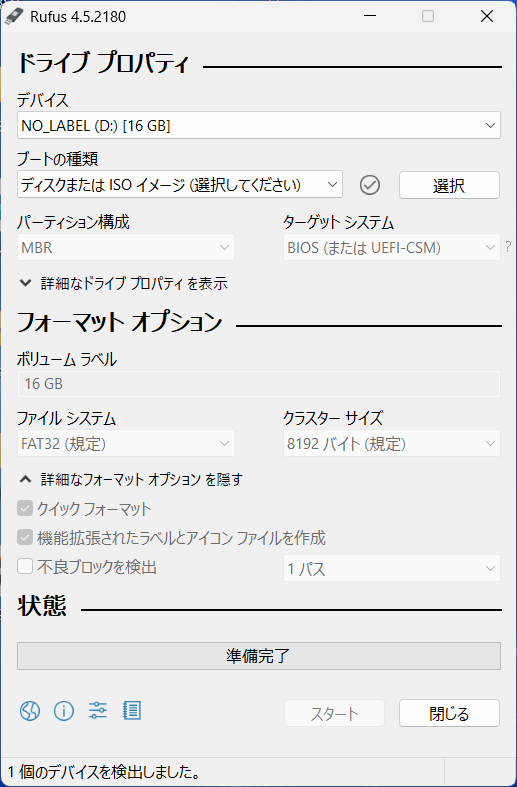
\includegraphics[width = 50mm]{rufus.png}
    \caption{rufusのウィンドウ}
  \end{center}
\end{figure}
\\
「選択」から先程ダウンロードしたUbuntuのisoファイルを選択して,スタートを選択する.これでUbuntuを起動する準備が整った.

\section{Ubuntuとの邂逅}
isoファイルを入れたUSBを挿し込んでBIOSを起動する.
そして,Bootの順位を変更してUbuntuを一番上に変更する.
これによりUbuntuが起動する.\\
まず初めに現時点では,Ubuntuに
IMEが導入されていないため日本語が入力できない.
これを解消するためにMozcをダウンロードしよう.\\
ターミナルを開いて以下を実行するとダウンロードが完了する.

\begin{tcolorbox}[terminalbox]
  \$ sudo apt update\\
  \$ sudo apt -y install ibus-mozc
\end{tcolorbox}


{\Huge
\textbf{忘れないうちに,ここで超重要なことを教えよう.}
\textbf{実行中のコマンドを強制終了するのはCtrl+cで行うことができる.}
}

\begin{subbox}{Mozcについて}

\end{subbox}


\begin{subbox}{-yについて}

\end{subbox}

\section{エディタ}
UNIX系のOSでは,viエディタが標準で搭載されている.
viエディタの基本的な使い方を紹介しよう.
\begin{tcolorbox}[terminalbox]
  \$ vi \textcolor{red}{ファイル名}
\end{tcolorbox}
\noindent とすれば,エディタが起動する.\\
viエディタは二つのモードが存在する.
\begin{center}
  \textbf{コマンドモード}$\rightleftarrows$ \textbf{インサートモード}
\end{center}
はじめに起動時には
\textbf{コマンドモード}になっている.
この状態では,テキストファイル内の文字列の編集はできず,入力された
文字はコマンドとして認識される.\\
とりあえず,覚えておくべきコマンドを紹介しよう.
\begin{enumerate}
  \item カーソル移動
  \begin{itemize}
    \item h\ :\ カーソルを一つ左に
    \item j\ :\ カーソルを一つ下に
    \item k\ :\ カーソルを一つ上に
    \item l\ :\ カーソルを一つ右に
    \item Ctrl+f\ : \ 次のページへ
    \item Ctrl+b\ : \ 前のページへ
  \end{itemize}
  \item 切り取り/コピー/貼り付け
  \begin{itemize}
    \item x\ :\ カーソル位置の文字を切り取る(ほとんどDeleteの意味)
    \item XX\ :\ カーソル位置の手前の文字を切り取る(ほとんどBackspaceの意味)
    \item dd\ :\ カーソルのある行の切り取り
    \item yy\ :\ カーソルのある行のコピー
    \item p\ :\ カーソルのある行の下に貼り付け
    \item P\ :\ カーソルのある行に貼り付け
  \end{itemize}
  \item ファイルの保存や終了など
  \begin{itemize}
    \item :w\ :\ ファイルの保存
    \item :w ファイル名\ :\ 名前をつけてファイルを保存
    \item :q\ :\ エディタの終了
    \item :wq\ :\ :wをして:qするコマンド(i.e. ファイルを保存して終了)
    \item !\ :\ 強制するコマンド.:q! $\leftarrow$ 強制終了, :wq! $\leftarrow$ 強制的に保存して終了
  \end{itemize}
\end{enumerate}
もちろん\textbf{インサートモード}に移行するコマンドが存在する.
インサートモードとはテキストを編集するモードのことである.
\begin{itemize}
  \item i\ :\ カーソルの位置からインサートモードに移行する.
  \item a\ :\ カーソルの後ろからインサートモードに移行する.
  \item o\ :\ カーソルのある行の下に空白行を追加してインサートモードに移行する.
\end{itemize}


\begin{subbox}{viとvim}

\end{subbox}



\chapter{Webサーバー}
\section{Apache}
本書では,WebサーバーとしてApacheを紹介する.\\
まず以下のコマンドでApacheをインストールしよう.
\begin{tcolorbox}[terminalbox]
  \$ sudo apt update
  \$ sudo apt -y install apache2
\end{tcolorbox}
インストールが完了したら早速Apacheを起動しよう!
\begin{tcolorbox}[terminalbox]
  \$ sudo systemctl start apache2
\end{tcolorbox}
これが起動コマンドである.
\begin{tcolorbox}[terminalbox]
  \$ sudo systemctl enable apache2
\end{tcolorbox}
これはApacheの自動起動の有効化を行うコマンドである.
\begin{tcolorbox}[terminalbox]
  \$ sudo systemctl status apache2
\end{tcolorbox}
これはApacheの現在の状態(ステータス)を表示するコマンドである.
ステータスのActiveの部分が\textcolor{green}{active(running)}になっていれば
Apacheが動いている.\\
最後に,ブラウザから「http://localhost」と入力すると
Apacheのウェルカムページ(Apache2 Default Pageと書かれたページ)が
表示されたら成功である.
\section{Apacheの設定}
Apacheの設定ファイルはサーバー全体に適応されるグローバル設定ファイル「/etc/apache2/apache2.conf」や
デフォルトでアクセスされる仮想ホストに適応される設定ファイル「/etc/apach2/sites-available/000-default.conf」で管理される.\\
仮想ホストに適応される設定ファイルについて変更を加えていこう.\\
まず,000-default.confの中身を以下に示す.(ただしコメントアウトは削除している.)
\begin{tcolorbox}[terminalbox]
  <VirtualHost *:80>\\
  \qquad ServerAdmin webmaster@localhost\\
  \qquad  DocumentRoot /var/www/html\\
  \qquad  ErrorLog \$\{APACHE\_LOG\_DIR\}/error.log\\
  \qquad  CustomLog \$\{APACHE\_LOG\_DIR\}/access.log combined\\
  </VirtualHost>
\end{tcolorbox}
上から見ていこう.
\begin{tcolorbox}[terminalbox]
  ServerAdmin webmaster@localhost
\end{tcolorbox}
とはApacheがエラー表示を行う場合などに問い合わせ先となる
連絡先メールアドレスまたは参照先URLを設定するのに使用.
\begin{tcolorbox}[terminalbox]
  DocumentRoot /var/www/html
\end{tcolorbox}
DocumentRootはWebページを配置するディレクトリである.この場合
Apacheのウェルカムページは/var/www/htmlディレクトリにあることがわかる.
\begin{tcolorbox}[terminalbox]
  ErrorLog \$\{APACHE\_LOG\_DIR\}/error.log
\end{tcolorbox}
はサーバーのエラーログをどこに保存するかを設定します.
\$\{APACHE\_LOG\_DIR\}は環境変数であって,Ubuntuにおいては
/etc/apache2/envvarsファイル内で定義されています.
私の実行環境では/var/log/apache2でした.
\begin{tcolorbox}[terminalbox]
  CustomLog \$\{APACHE\_LOG\_DIR\}/access.log combined
\end{tcolorbox}
はサーバーのアクセスログをどこに保存するかを設定します.
combinedは,アクセスログのフォーマットを指定するもの.\\
また,
\begin{tcolorbox}[terminalbox]
  DirectoryIndex \textcolor{red}{ファイル名}
\end{tcolorbox}
で表示するhtmlファイルを指定することができる.

\subsection{仮想ホストの作成}
「/etc/apache2/sites-available/000-default.conf」が初期の仮想ホスト
として設定されている.これを残したまま別の仮想ホストを作成する
場合は,「/etc/apache2/sites-available/」直下に新たな設定ファイルを作成する.\\
簡単のために,もとあった000-default.confをコピーするとよい.
\begin{tcolorbox}[terminalbox]
  \$ sudo cp \textcolor{red}{コピーするファイル} \textcolor{red}{コピーした後のファイル名}
\end{tcolorbox}
なので,今回はtest.confという設定ファイルを作成しよう.
\begin{tcolorbox}[terminalbox]
  \$ sudo cp \textcolor{red}{/etc/apache2/sites-available/000-default.conf} \textcolor{red}{/etc/apache2/sites-available/test.conf}
\end{tcolorbox}
次に,DocumentRootとDirectoryIndexを変更しよう.
今回は以下のように設定した.
\begin{tcolorbox}[terminalbox]
  <VirtualHost *:80>\\
  \qquad ServerAdmin webmaster@localhost\\
  \qquad DocumentRoot /hoge\\
  \qquad DirectoryIndex hoge.html
  \qquad ErrorLog \$\{APACHE\_LOG\_DIR\}/error.log\\
  \qquad CustomLog \$\{APACHE\_LOG\_DIR\}/access.log combined\\
  </VirtualHost>
\end{tcolorbox}
ディレクトリやファイルを作成しよう.
\begin{tcolorbox}[terminalbox]
  \$ sudo mkdir /hoge
\end{tcolorbox}
\begin{tcolorbox}[terminalbox]
  \$ sudo touch /hoge/hoge.html\\
  \$ sudo vi /hoge/hoge.html
\end{tcolorbox}
で適当なhtmlファイルを作成する.\\
次に作成した仮想ホストを有効化したい
有効化する前に今有効になっているデフォルトの仮想ホストを切断しよう.
\begin{tcolorbox}[terminalbox]
  \$ sudo a2dissite 000-default.conf
\end{tcolorbox}
次にこの設定をサーバーに反映させるためにリロードしよう.
\begin{tcolorbox}[terminalbox]
  \$ sudo systemctl reload apache2
\end{tcolorbox}
さて,先ほど作成した仮想ホストを有効化しよう.
\begin{tcolorbox}[terminalbox]
  \$ sudo a2ensite \textcolor{red}{test.conf}
\end{tcolorbox}
次に有効化した仮想ホストをサーバーに反映させよう.
\begin{tcolorbox}[terminalbox]
  \$ sudo systemctl reload apache2
\end{tcolorbox}
いま,「http://localhost」にアクセスしたら「403 Forbidden」が表示されるはずだ.
これを解消するためにグローバル設定ファイル(/etc/apache2/apache2.conf)
を編集しよう.
以下のように書かれている部分をみよう.
\begin{tcolorbox}[terminalbox]
  <Directory /www/html>\\
  \qquad Options Indexes FollowSymLinks\\
  \qquad AllowOverride None\\
  \qquad Require all granted\\
  </Directory>
\end{tcolorbox}
これはデフォルトのDocumentRootに対する設定であって,
\begin{tcolorbox}[terminalbox]
  <Directory /www/html>
\end{tcolorbox}
を
\begin{tcolorbox}[terminalbox]
  <Directory /hoge>
\end{tcolorbox}
に変更して
\begin{tcolorbox}[terminalbox]
  \$ sudo systemctl reload apache2
\end{tcolorbox}
設定を反映させよう.
\begin{subbox}{403 Forbidden}
  今回なぜ403 Forbiddenが出たのかと言うと,Apacheが/hogeにアクセスする権限がないためである.そのため/hogeにアクセスしてもいいですよ.
  ということを先ほどの設定でする必要がある.
\end{subbox}

\subsection{ファイアーウォールの設定}
Ubuntuでは,ファイアーウォールは\textbf{ufwコマンド}を用いる.
\begin{tcolorbox}[terminalbox]
  \$ sudo ufw enable
\end{tcolorbox}
これでファイアーウォールを有効化
\begin{tcolorbox}[terminalbox]
  \$ sudo ufw allow Apache
\end{tcolorbox}
80番ポートの開放
\begin{tcolorbox}[terminalbox]
  \$ sudo ufw status
\end{tcolorbox}
これでufwの状態を確認することができる.\\
うまく行っていればToの下にApache,Apache(v6),Actionの下にALLOW,Fromの下に
Anywhere,Anywhere(v6)と出るはずである.


\chapter{Docker}
さてDockerのインストールから早速行う  .
\begin{tcolorbox}[terminalbox]
  \$ sudo apt update
\end{tcolorbox}
お決まりのアップデート
\begin{tcolorbox}[terminalbox]
  \$ sudo apt install ca-certificates curl
\end{tcolorbox}
ca-certificatesとcurlのインストールである.
\begin{tcolorbox}[terminalbox]
  \$ sudo install -m 0755 -d /etc/apt/keyrings
\end{tcolorbox}
\begin{tcolorbox}[terminalbox]
  \$ sudo curl -fsSL https://download.docker.com/linux/ubuntu/gpg -o /etc/apt/keyrings/docker.asc
\end{tcolorbox}
\begin{tcolorbox}[terminalbox]
  \$ sudo chmod a+r /etc/apt/keyrings/docker.asc
\end{tcolorbox}
\begin{tcolorbox}[terminalbox]
  \$ echo "deb [arch=\$(dpkg --print-architecture) signed-by=/etc/apt/keyrings/docker.asc] https://download.docker.com/linux/ubuntu \$(./etc/os-release \&\& echo "\$VERSION\_CODENAME") stable" | sudo tee /etc/apt/sources.list.d/docker.list > /dev/null
\end{tcolorbox}

\begin{tcolorbox}[terminalbox]
  \$ sudo apt update
\end{tcolorbox}
\begin{tcolorbox}[terminalbox]
  \$ sudo apt install docker-ce docker-ce-li containerd.io docker-buildx-plugin docker-compose-plugin
\end{tcolorbox}
Dockerのインストールが完了したことを確認するためにバージョンと状態確認を行う.
\begin{tcolorbox}[terminalbox]
  \$ sudo docker --version\\
  \$ sudo systemctl status docker
\end{tcolorbox}

\section{Dockerを使う}
以下のコマンドでコンテナを起動する.
\begin{tcolorbox}[terminalbox]
  \$ docker container run \textcolor{red}{IMAGE}
\end{tcolorbox}
さてHello Worldに相当するものを実行してみよう.

\begin{tcolorbox}[terminalbox]
  \$ docker container run hello-world
\end{tcolorbox}
実行すれば,チュートリアルやドキュメントのURLが記載されてるものが出てくるだろう.\\
コンテナ一覧を確認するには
\begin{tcolorbox}[terminalbox]
  \$ docker container ls
\end{tcolorbox}
を実行する.

\section{Dockerを用いたWebサーバー}
httpdというイメージを用いてコンテナを起動することでWebサーバーを起動することができる.まずサーバー管理用のディレクトリを作成しよう.
\begin{tcolorbox}[terminalbox]
  \$ mkdir -p $\sim$/dockertest/htdocs $\sim$/dockertest/conf
\end{tcolorbox}
次にhttpdコンテナを起動しよう.
\begin{tcolorbox}[terminalbox]
  \$ cd $\sim$/dockertest\\
  \$ docker run -dit --name my-apache-app -p 8080:80 -v ./htdocs:/usr/local/apache2/htdocs/ -v ./conf:/usr/apache2/conf httpd:2.4
\end{tcolorbox}
「-v ./htdocs:/usr/apache2/htdocs/」や「-v ./conf:/usr/apache2/conf」によって
「$\sim$/dockertest/htdocs」や「$\sim$/dockertest/conf」に配置されたファイルがコンテナに反映されるようになる.
例えば,「$\sim$/dockertest/htdocs」の直下にindex.htmlを配置すると,その内容がアクセス時に表示される.




\chapter{参考文献}

\begin{itemize}
  \item \url{https://www.miraiserver.ne.jp/column/about\_ubuntu-ufw/}
  \item \url{https://xtech.nikkei.com/it/article/COLUMN/20060228/231037/}
  \item \url{https://qiita.com/erik\_t/items/d8f4746d2dc2992f329e}
  \item \url{https://www.apache.org/}
  \item \url{https://uchy.me/blog/20240815024/}
  \item \url{https://www.javadrive.jp/apache/}
  \item \url{https://qiita.com/moko\_Swallows/items/be918efda9cfebcbf6b6}
  \item \url{https://www.miraiserver.ne.jp/column/about\_vi-editor/}
  \item \url{https://ferret-one.com/blog/403}
  \item \url{https://viva-linux.jp/linux-mint-japanese-input-mozc-211}
  \item \url{https://qiita.com/SatoshiSobue/items/a612ebbb3a9242c09db5}
  \item \url{https://www.kagoya.jp/howto/cloud/container/docker/}
  \item \url{https://ubuntu.com}
  \item \url{https://blog.kabocy.com/linux/5806/}
\end{itemize}


\appendix
\chapter{コマンド一覧}
気が向けばコマンドについての一覧を作る.


\end{document}
